\documentclass[11pt]{article}
\addtolength{\oddsidemargin}{-1.cm}
\addtolength{\textwidth}{2cm}
\addtolength{\topmargin}{-2cm}
\addtolength{\textheight}{3.5cm}
\newcommand\tab[1][1cm]{\hspace*{#1}}
\usepackage[pdftex]{graphicx}
\usepackage{pdflscape}
\usepackage[T1]{fontenc}
\usepackage{hyperref}
\usepackage{float}
\usepackage{cite}
\hypersetup{
	colorlinks=true,
	linkcolor=black,
	filecolor=magenta,
	urlcolor=cyan,
}

% define the title
\author{Panda Inc}
\title{Architectural Design Document}
\begin{document}
\begin{titlepage}

	\begin{center}
		% Upper part of the page
        
\includegraphics[width=0.7\linewidth]{images/panda.jpg}\\[1cm]
		\textsc{\LARGE Momentum - Multipy Active Dayz App}\\[0.3cm]
		% Title
		\rule{\linewidth}{0.5mm} \\[1cm]
		{ \huge \bfseries Architectural Design Document}\\[0.5cm]
		\rule{\linewidth}{0.5mm} \\[1cm]


		\begin{minipage}{0.4\textwidth}
			\begin{flushleft} \large
				\emph{} \\
				Quinton {Swanepoel}
			\end{flushleft}
		\end{minipage}
		\begin{minipage}{0.4\textwidth}
			\begin{flushright} \large
				\emph{} \\
				15245510
			\end{flushright}
		\end{minipage}

		\begin{minipage}{0.4\textwidth}
			\begin{flushleft} \large
            	\emph{} \\
				Azhar {Patel}
			\end{flushleft}
		\end{minipage}
		\begin{minipage}{0.4\textwidth}
			\begin{flushright} \large
				\emph{} \\
				15052592
			\end{flushright}
		\end{minipage}

		\begin{minipage}{0.4\textwidth}
			\begin{flushleft} \large
				\emph{} \\
				Tshepo Macebo {Malesela}
			\end{flushleft}
		\end{minipage}
		\begin{minipage}{0.4\textwidth}
			\begin{flushright} \large
				\emph{} \\
				14211582
			\end{flushright}
		\end{minipage}

        \begin{minipage}{0.4\textwidth}
			\begin{flushleft} \large
				\emph{} \\
				Keaton {Pennels}
			\end{flushleft}
		\end{minipage}
		\begin{minipage}{0.4\textwidth}
			\begin{flushright} \large
				\emph{} \\
				14373018
			\end{flushright}
		\end{minipage}

		\rule{\linewidth}{0.5mm} \\[1cm]
		\textsc{\Large Stakeholders}\\[1cm]

		\begin{minipage}{0.4\textwidth}
			\begin{flushleft} \large
				\emph{} \\
				MMI Holdings:
			\end{flushleft}
		\end{minipage}
		\begin{minipage}{0.4\textwidth}
			\begin{flushright} \large
				\emph{} \\
				Phillip Kruger
			\end{flushright}
		\end{minipage}


	\end{center}
\end{titlepage}

\newpage
\paragraph{Abstract}\mbox{}\\
This document serves to describe the architecture used for the ActiveDayz application which is developed for Momentum (Multiply) as part of the Software Engineering Project (COS 301) at the University of Pretoria.\newline
The document complies with the Architectural Design Document Software Engineering Standard, as set by the European Space Agency.



\newpage
\tableofcontents

\newpage

\section{Introduction}
\subsection{Purpose}
Active Dayz is part of Momentum's Multiply wellness and rewards programme. The Active Dayz programme tracks a user's steps taken and calories burned in order to provide users with relevant rewards. The programme currently only works with certain devices. An application is required that can log events such as marathons and other fitness events that users may attend, monitor users gym time, and track users steps taken and calories burned.

\subsection{Scope}
Active Dayz is aimed at providing momentum customers  with a quick way to get rewards/active days by making use of location based services to track when a user goes to gym and how long they stay for.
\newline
\newline
The proposed system is to be integrated with a non-existing admin web interface. It should allow the integration of various services of which location based monitoring is the main objective. Other tools may include monitoring of steps take, calories burned and events attended.

\subsection{Definitions and Abbreviations}
\subsubsection{Definitions}
\subsubsection{Abbreviations}

\subsection{References}
\subsection{Overview}
\newpage
\section{Architectural Design}
\subsection{Deployment Diagram}
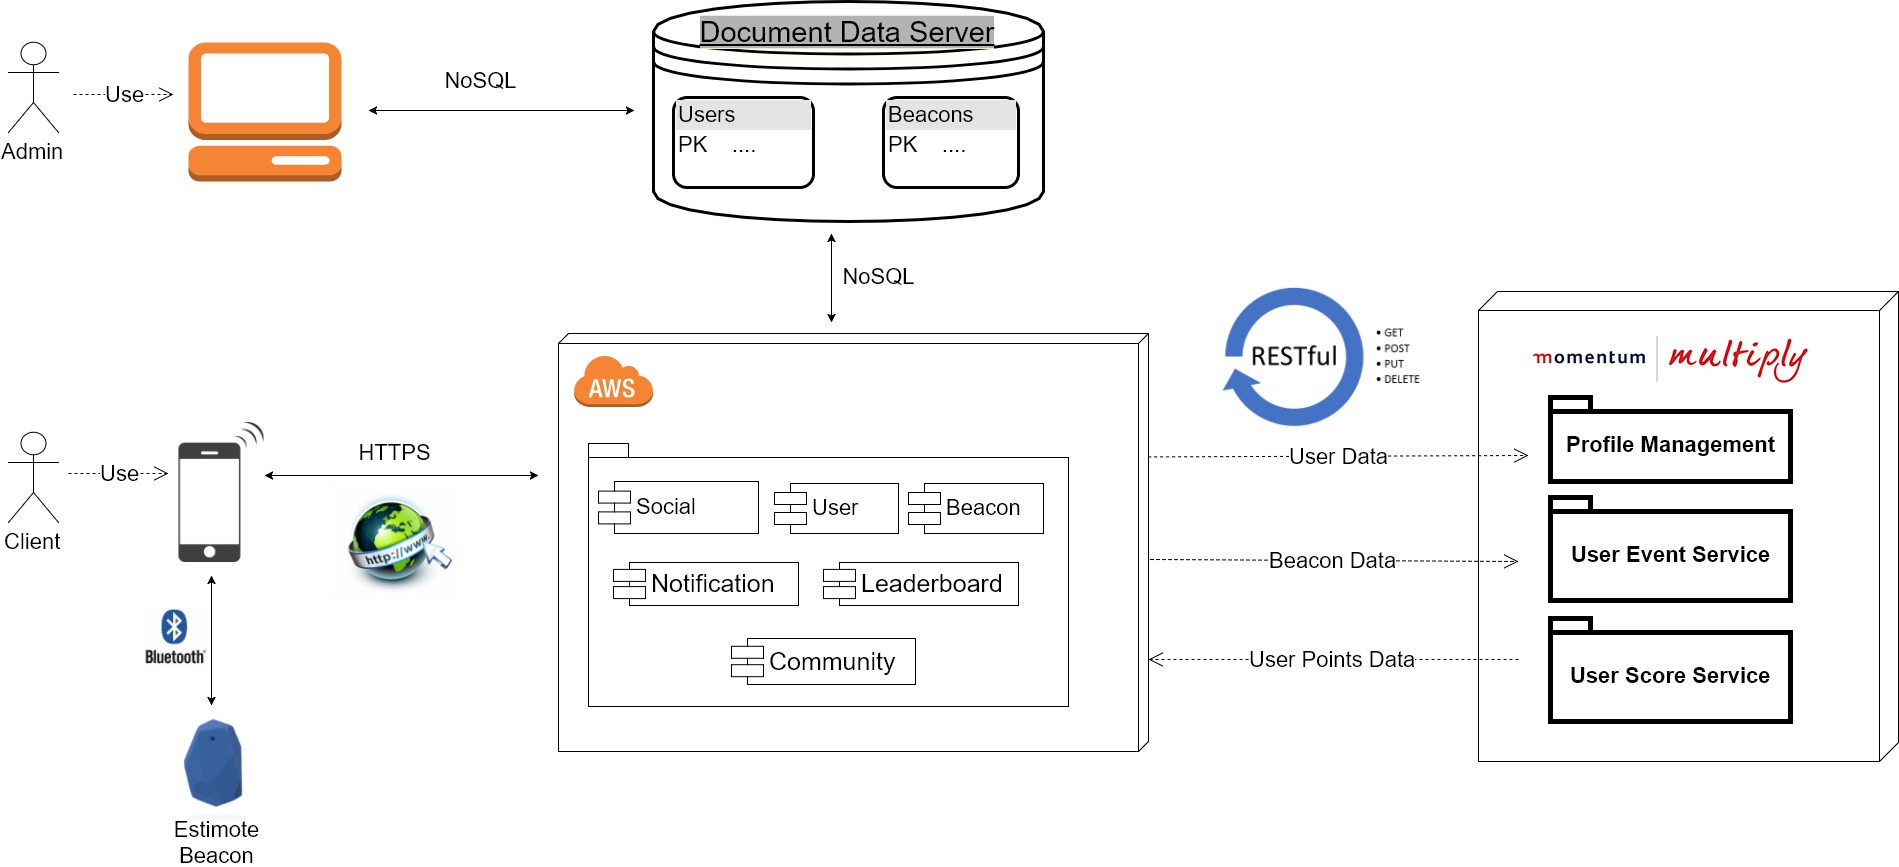
\includegraphics[width=175mm, scale=1.5]{images/Deployment.jpg}\\[1cm]
\subsection{Architectural Patterns of ActiveDayz}
\begin{itemize}
\item Service oriented architecture patterns (Micro services)
\item Layered architecture patterns
\item Event-Driven patterns
\end{itemize}
The first two design patterns were chosen such that the modules within our application would have the as few as possible and also so that we could ensure we achieve low coupling. The event driven pattern will aid in the connecting and ranging of the event driven beacons

\subsection{Non Functional Requirements }
Listed below are the 3 non functional requirements which have been collectively identified by the us, the development team, and our client as those which are required during the development of the ActiveDayz application.
\begin{enumerate}
  \item \emph{Security Requirements:} This refers to the protection of our systems data and the system itself. In terms of protection of the system related data, identification and authentication of Multiply clients has been identified as a process of importance. This has been accommodated for in the Users Module. In terms of securing the system, the system will be deployed and hosted on a trusted COTS server, Amazon Web Service Elastic Compute Cloud (EC2) and communication channels over the network will be secured using SSH
  \item \emph{Quality Requirements:} 
	\begin{enumerate}
		\item Reliability - The system will be designed such that it will behave consistently in a user-acceptable manner when in operation. The EC2 server provides some of this capability through load balancing during periods of elevated requests for system resources. 
		\item Maintainability - The software of our application will be produced such that it requires minimal effort to update or modify components. The use of a micro service architecture will facilitate this requirement and in addition, the system will be designed to be testable through the use of a comprehensive testing structure in order to ensure accurate functionality after modification 
		\item Availability
	\end{enumerate}
	\item \emph{Interface Requirements -} Interfacing, and the interaction behavior of clients with the application was highlighted as an area of importance during development external entities to communicate with the system. The layout, look and feel will be designed according to the guidelines given by the client. The guidelines relate to how the above mentioned attributes have been applied in other Multiply applications/websites and are considerations which we as the design team need to heed of 

\end{enumerate}
[\textit{Please note, this does not represent an exhaustive list of the non functional requirements. These are to be further updated}]


\subsection{Design Requirements }
\begin{itemize}
\item Our goal is to design a highly modular system which has minimal dependency between the modules
\item The system is required to be designed such that if a module needs to be updated/modified or if a module needs to be added or removed. that this can be done with minimal effort
\end{itemize}
\subsection{Design Constraints}
The following design constraints are combination of those which were stipulated in the client's application for the call for projections and those which have been identified during meetings. These have been put it place in order to ensure seamless integration of the application into their already existing business structure
\begin{itemize}
\item Java EE to used for back-end development
\item A non relational Database used to store data about the user (graph or document)
\item Cloud Services in order to host the back-end services 
\item Containers in order to deploy the application 
\item The use of beacons in order to facilitate location based functionality
\end{itemize}

\section{Component Descriptions}
\subsection{Beacon Module}
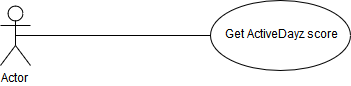
\includegraphics[width=0.7\linewidth]{images/Beacon.png}\\[1cm]
\subsection{Notification Module}
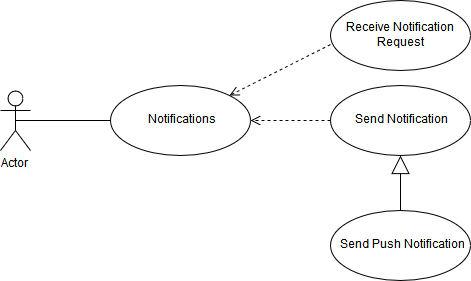
\includegraphics[width=0.7\linewidth]{images/Notification.png}\\[1cm]
\subsection{Leader Module}
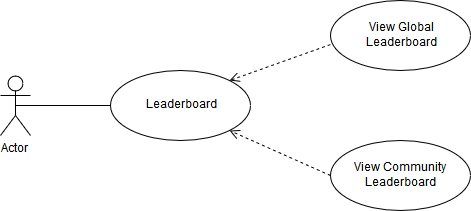
\includegraphics[width=0.7\linewidth]{images/Leaderboard.png}\\[1cm]
\subsection{Community Module}
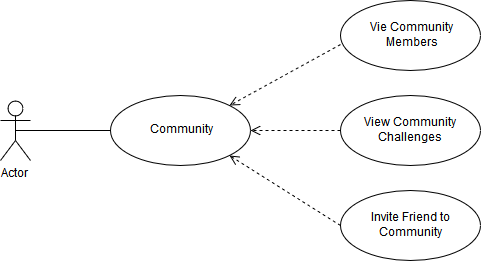
\includegraphics[width=0.7\linewidth]{images/Community1.png}\\[1cm]
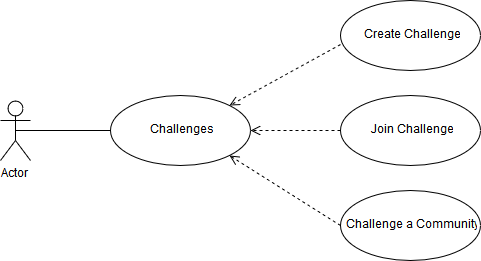
\includegraphics[width=0.7\linewidth]{images/Community2.png}\\[1cm]
\subsection{Users Module}
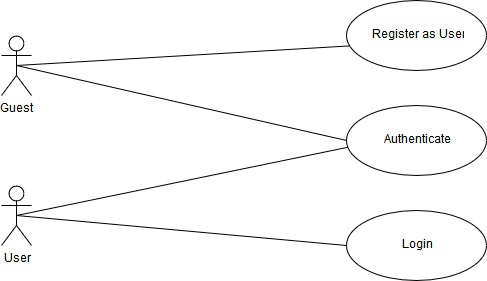
\includegraphics[width=0.7\linewidth]{images/UserManagement.png}\\[1cm]
\subsection{Social Module}
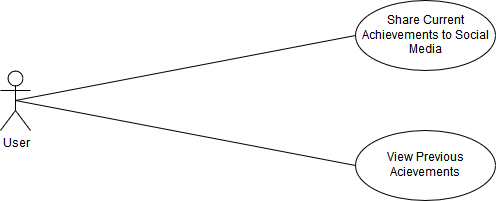
\includegraphics[width=0.7\linewidth]{images/Social.png}\\[1cm]

\section{Integration Diagram}
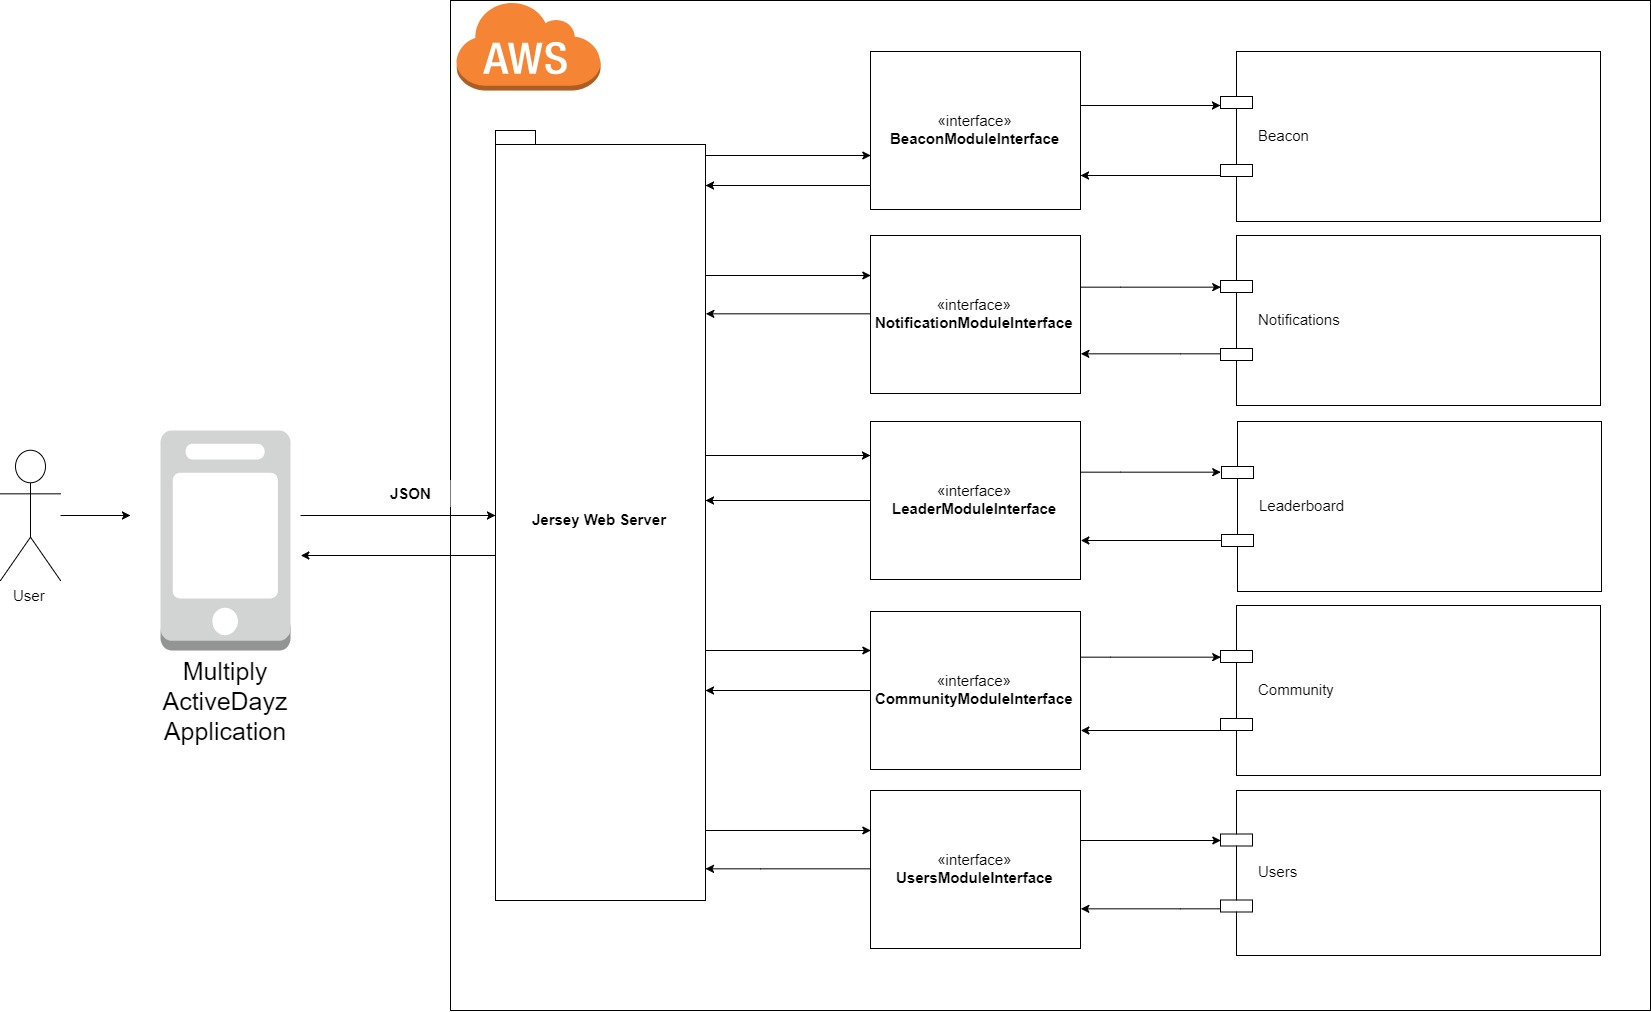
\includegraphics[width=175mm, scale=1.5]{images/Integration.jpg}\\[1cm]
\section{Feasibility and Resource Estimates}

\section{Technologies Used}
\subsection{Server}
\textbf{JavaEE} ( eclipse oxygen ) will be used as the language to develop the server. The server will will implement \textbf{Jersey RESTful} web services as a means of accessing the various modules described above.
\newline
The server will be contained within a \textbf{Tomcat 8} application server and all of these components will be hosted on an \textbf{Amazon Web Service Elastic Cloud Computing} instance
\newline
\textbf{Maven} will be used for compilation, build and testing automation. Finally communication between modules will be structured using \textbf{JSON} in order to ensure low coupling between modules 
\subsection{Web develpement}
polymer\\
node bower and polymer\\
js\\
mysql db\\
beacons estimotes\\
docker\\
wildfly\\

\end{document}
